\frame{\titlepage}

\begin{frame}
  \frametitle{Краткая история проекта}
  \framesubtitle{1970--1980-е гг.}

  \begin{block}{}
    \begin{itemize}
      \item создание кафедрального фонда фото- и ксерокопий списков севернорусских житий и похвальных слов XV--XVII~вв.\autocite{averina_alexeeva_gerd:1996}
      \item перевод в машиночитаемый формат при помощи 8-битной кодировки на базе ASCII и специальных правил транслитерации
      \item версия Unicode 1.0 появилась в 1991~г., а все недостающие выносные~--- в версии 6.1 блока Cyrillic Extended-B (2012~г.)
    \end{itemize}
  \end{block}
\end{frame}

\begin{frame}
  \frametitle{Транслитерация}
  \framesubtitle{Житие Корнилия Комельского, 88~об.}

  \begin{columns}[c]
    \begin{column}{6cm}
      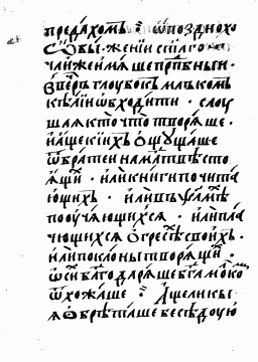
\includegraphics[width=5cm]{KK_src}
    \end{column}

    \begin{column}{6cm} \ttfamily \footnotesize
      \textcolor{gray}{Z -88} ПPEДAXOMЪ. W ПOЗДHOXO\& \\
      ЖEHIИ CTAГO\#. WБЫ\& \\
      ЧAИ ЖE ИMRШE ПPП(Д)БHЫИ.\& \\
      B BE(ч)PЪ ГЛUБOKЪ MЛЪKOMЪ\& \\
      K+ЛIИ WБXOДИTИ. CЛU\& \\
      ШAR KTO ЧTO TBOPRШE.\& \\
      И AЩE KIИXЪ OЩDЩAШE\& \\
      W(Т) БPATEИ HA MЛTB+\# CTO\& \\
      RЩИ(X). ИЛИ KHИГИ ПOЧИTA\& \\
      ЮЩИXЪ. ИЛИ BЪ QЛM+(X)\#\& \\
      ПOUЧRЮЩИXCR. ИЛИ ПЛA\& \\
      ЧЮЩИXCR O ГPEC+(X) CBOИXЪ.\& \\
      ИЛИ ПOKЛOHЫ TBOPRЩИ(X).\& \\
      W CИ(X) БЛГOДAPRШE\# БГA\# MО(л)KO(M)\& \\
      W(Т)XOЖAШE. AЩE ЛИ KЫ\& \\
      R OБP+TAШE БEC+ДUЮ \textcolor{gray}{Z 89 ЩИXЪ}
    \end{column}
  \end{columns}
\end{frame}

\begin{frame}
  \frametitle{Правила транслитерации}

  \begin{block}{Графемы}
    \begin{table}
      \begin{tabularx}{\textwidth}{XXXXXXXXXXXXXX}
        \texttt{I} & \texttt{R} & \texttt{V} & \texttt{W} & \texttt{U} & \texttt{+} & \texttt{F} &
        \texttt{S} & \texttt{G} & \texttt{D} & \texttt{L} & \texttt{Q} & \texttt{Я} & \texttt{\$} \\
        {\agio ї} & {\agio ѧ} & {\agio ѵ} & {\agio ѡ} & {\agio ѹ} & {\agio ѣ} & {\agio ѳ} &
        {\agio ѕ} & {\agio ѫ} & {\agio ꙋ} & {\agio ѯ} & {\agio ѱ} & {\agio ꙗ} & {\agio ҂} \\
      \end{tabularx}
    \end{table}
  \end{block}

  \begin{block}{Надстрочные знаки}
    \begin{table}
      \begin{tabularx}{\textwidth}{XXX}
        Титло & \texttt{СТАГО\#} & {\agio ст҃аго} \\
        Буквотитло & \texttt{BE(ч)PЪ} & {\agio ве҇ⷱръ} \\
        Выносная буква & \texttt{ГРЕС+(Х)} & {\agio гресѣⷯ} \\
      \end{tabularx}
    \end{table}
  \end{block}

  \begin{block}{Переносы}
      \texttt{\&}~--- новая строка,
      \texttt{\textbackslash}~--- столбец,
      \texttt{Z -?\textbackslash{}d+} --- страница
  \end{block}

  % Знаки препинания, имена собственные
\end{frame}

\begin{frame}
  \frametitle{Краткая история проекта}
  \framesubtitle{1990--2000-е~гг.}

  \begin{block}{}
    \begin{itemize}
      \item публикация серии <<Памятники русской агиографической литературы>>\autocite{coll:2012}
      \item выход в онлайн: \url{http://project.phil.spbu.ru/scat/}
      \item XML-представление рукописей на основе рекомендаций консорциума TEI\autocite{alexeev:2009}
      \item разработка и апробация формата морфологической разметки\autocite{ivanova:2006}
    \end{itemize}
  \end{block}
\end{frame}

\begin{frame}
  \frametitle{Памятники русской агиографической литературы}

  \begin{center}
    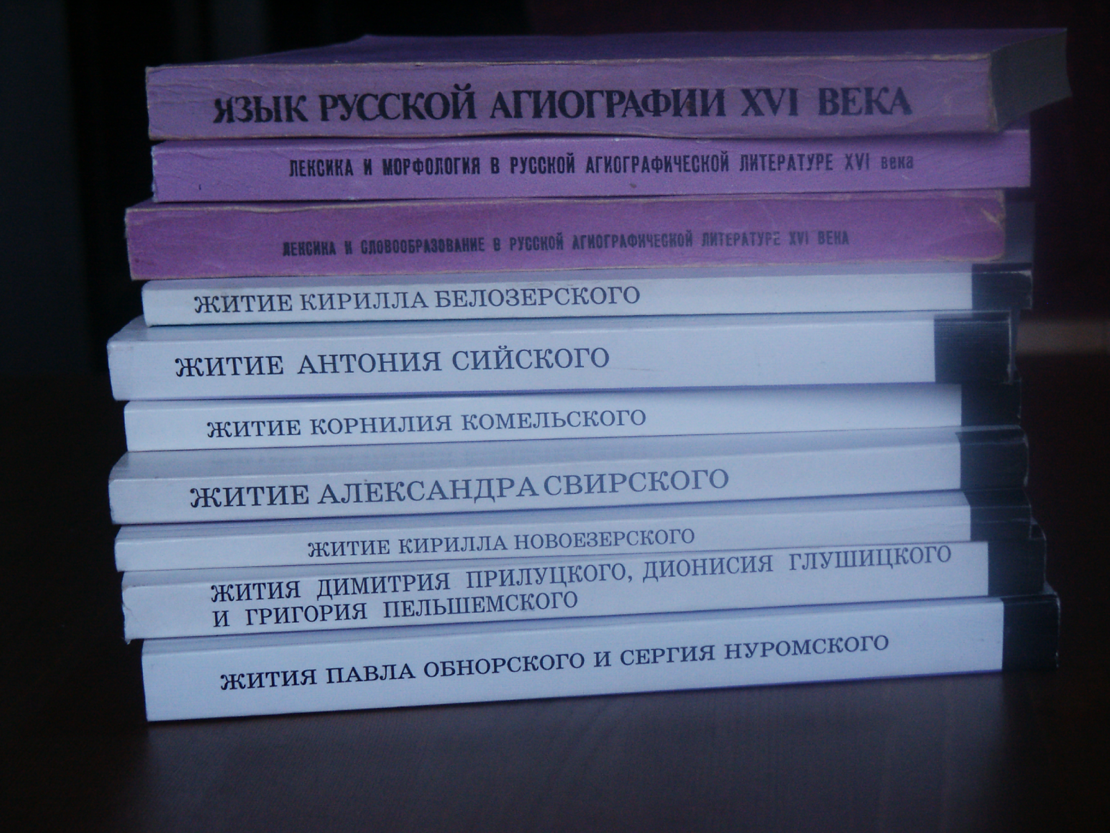
\includegraphics[width=0.7\linewidth]{books}
  \end{center}
\end{frame}

\begin{frame}
  \frametitle{XML}
  \framesubtitle{eXtensible Markup Language}

  \begin{center}
    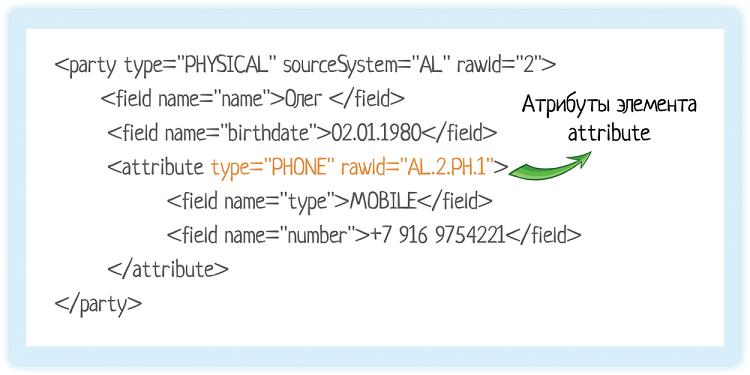
\includegraphics[width=\linewidth]{xml}
  \end{center}
\end{frame}

\begin{frame}
  \frametitle{TEI}
  \framesubtitle{Text Encoding Initiative}

  \begin{center}
    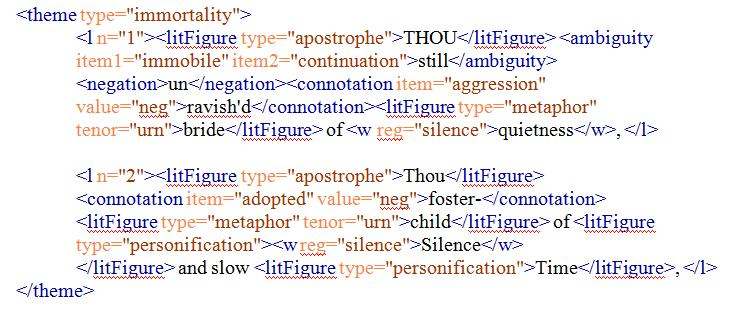
\includegraphics[width=\linewidth]{tei}
  \end{center}
\end{frame}

\begin{frame}[fragile]
  \frametitle{PDF и XML}

  \begin{columns}[c]
    \begin{column}{6cm}
      
\includegraphics[width=\linewidth]{CN_pdf}
    \end{column}

    \begin{column}{6cm}
      \begin{Verbatim}[fontsize=\footnotesize]
<pb n="-25"/>
<lb n="1"/>
<w lemma="м+сяць"
   msd="jo;род;ед;м"
   pos="сущ"
   reg="м+сяца"
   src="М+СRЦА"
   xml:id="CrlNvz.0">
  мѣсѧца</w>
<lb n="2"/>
<w lemma="февруарии"
   msd="jo;род;ед;м"
   pos="сущ"
   reg="февруария"
   src="ФЕVРDАРIА"
   xml:id="CrlNvz.1">
  феѵрꙋарїа</w>
\end{Verbatim}
    \end{column}
  \end{columns}
\end{frame}

\begin{frame}
  \frametitle{Морфологический анализ исторических текстов}
  \framesubtitle{Проблемы}

  \begin{enumerate}
    \item малый объём текстов
    \item<2-> орфографическая нормализация
    \item<3-> разные кодировки, разные коллективы\ldots
  \end{enumerate}

  \onslide<2>
  \begin{columns}[c]
    \begin{column}{5cm}
      \begin{itemize}
        \item {\agio блаженаго}
        \item {\agio блаженна҇ⷢ}
        \item {\agio бл҃жена҇ⷢ}
      \end{itemize}
    \end{column}

    \begin{column}{5cm}
      \begin{itemize}
        \item {\agio бл҇ⷶженнаго}
        \item {\agio бл҃женⷩаго}
        \item {\agio бла҇ⷤнна҇ⷢ}
      \end{itemize}
    \end{column}
  \end{columns}
\end{frame}

\begin{frame}
  \frametitle{Морфологический анализ исторических текстов}
  \framesubtitle{Подходы}

  \begin{block}{}
    \begin{enumerate}
      \item<1-> ручной \begin{itemize}
        \item древнерусский подкорпус НКРЯ (500 тыс.\ с/у)
        \item подкорпус древнерусских берестяных грамот (20 тыс.\ с/у)
        \item \alert<4->{СКАТ} (500 тыс.\ с/у)
      \end{itemize}
      \item<2-> на основе грамматического словаря \begin{itemize}
        \item церковнославянский подкорпус НКРЯ (4,7 млн с/у)
        \item старорусский подкорпус НКРЯ (7 млн с/у)
        \item система <<Манускрипт>> (3,5 млн с/у)
      \end{itemize}
      \item<3-> другие подходы \begin{itemize}
        \item проецирование разметки с современных языков
        \item нейросети
      \end{itemize}
    \end{enumerate}
  \end{block}
\end{frame}

\begin{frame}
  \frametitle{Спецификация формата разметки}

  \begin{center}
    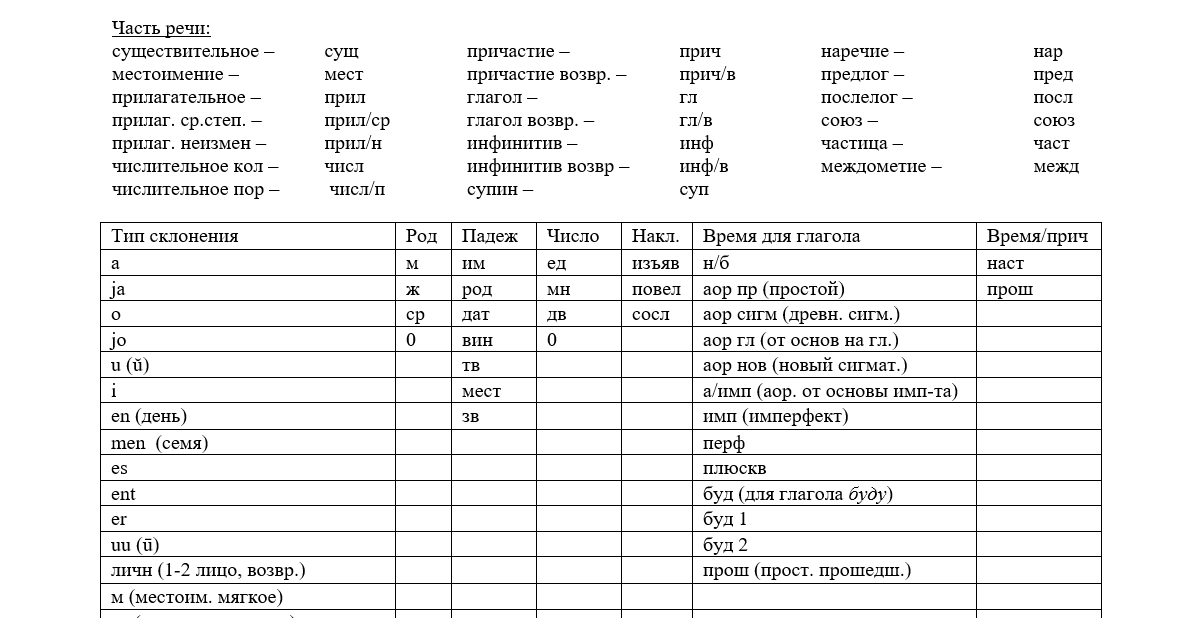
\includegraphics[width=0.9\linewidth]{spec}
  \end{center}
\end{frame}

\begin{frame}
  \frametitle{Настоящее и будущее проекта}
  \framesubtitle{2010--2020-е~гг.}

  \begin{block}{Морфология}
    \begin{itemize}
      \item морфологическая разметка 5 житий ($\sim$50~тыс.\ с/у)
      \item лемматизация и полуавтоматическая разметка\autocite{sipunin:2020}
    \end{itemize}
  \end{block}
\end{frame}

\begin{frame}
  \frametitle{Размеченные тексты}

  \footnotesize \setlength{\aboverulesep}{0.5pt} \setlength{\belowrulesep}{0.5pt}
  \begin{tabularx}{\textwidth}{Xp{0.75cm}p{0.75cm}p{0.75cm}p{0.75cm}p{0.75cm}p{0.75cm}}
    \toprule
    \texttt{М(с)ЦА} & сущ  & jo & род & ед & м  &    \\ \midrule
    \texttt{IЮНR} & сущ  & jo & род & ед & м  &    \\ \midrule
    \texttt{ДНЬ\#} & сущ  & en & им  & ед & м  &    \\ \midrule
    \texttt{А\#} & 1    &    &     &    &    &    \\ \midrule
    \texttt{ЖИТIЕ} & сущ  & jo & им  & ед & ср &    \\ \midrule
    \texttt{И} & союз &    &     &    &    &    \\ \midrule
    \texttt{ПОДВИЗИ} & сущ  & о  & им  & мн & м  & *  \\ \midrule
    \texttt{И} & союз &    &     &    &    &    \\ \midrule
    \texttt{W(Т)ЧАСТИ\&} & нар  &    &     &    &    &    \\ \midrule
    \texttt{ЧЮДЕ(с)} & сущ  & es & род & мн & ср &    \\ \midrule
    \texttt{ИСПОВ+ДА(н)Е} & сущ  & jo & им  & ед & ср & +и \\ \midrule
    \texttt{ПРП(Д)БНА(г)} & прил & тв & род & ед & м  &    \\ \midrule
    \texttt{W(ц)} & сущ  & jo & род & ед & м  &    \\ \midrule
    \texttt{НШЕ(г)} & мест & м  & род & ед & м  &    \\ \midrule
    \texttt{*ДIОНIСIА} & сущ  & jo & род & ед & м  &    \\ \midrule
    \texttt{*ГЛD(ШИ)ЦКА(г);\&} & прил & тв & род & ед & м  &    \\ \bottomrule
  \end{tabularx}
\end{frame}

\begin{frame}
  \frametitle{Размеченные тексты + лемматизация}

  \footnotesize \setlength{\aboverulesep}{0.5pt} \setlength{\belowrulesep}{0.5pt}
  \begin{tabularx}{\textwidth}{XXp{0.75cm}p{0.75cm}p{0.75cm}p{0.75cm}p{0.75cm}p{0.75cm}}
    \toprule
    \texttt{М(с)ЦА} & \texttt{МЕСЯЦЬ}                & сущ  & jo & род & ед & м  &    \\ \midrule
    \texttt{IЮНR} & \texttt{ИЮНЬ}                    & сущ  & jo & род & ед & м  &    \\ \midrule
    \texttt{ДНЬ\#} & \texttt{ДЕНЬ}                   & сущ  & en & им  & ед & м  &    \\ \midrule
    \texttt{А\#} &                                   & 1    &    &     &    &    &    \\ \midrule
    \texttt{ЖИТIЕ} & \texttt{ЖИТИЕ}                  & сущ  & jo & им  & ед & ср &    \\ \midrule
    \texttt{И} & \texttt{И}                          & союз &    &     &    &    &    \\ \midrule
    \texttt{ПОДВИЗИ} & \texttt{ПОДВИГЪ}              & сущ  & о  & им  & мн & м  & *  \\ \midrule
    \texttt{И} & \texttt{И}                          & союз &    &     &    &    &    \\ \midrule
    \texttt{W(Т)ЧАСТИ\&} & \texttt{ОТЧАСТИ}          & нар  &    &     &    &    &    \\ \midrule
    \texttt{ЧЮДЕ(с)} & \texttt{ЧЮДО}                 & сущ  & es & род & мн & ср &    \\ \midrule
    \texttt{ИСПОВ+ДА(н)Е} & \texttt{ИСПОВ+ДАНИЕ}     & сущ  & jo & им  & ед & ср & +и \\ \midrule
    \texttt{ПРП(Д)БНА(г)} & \texttt{ПРЕПОДОБНЫИ}     & прил & тв & род & ед & м  &    \\ \midrule
    \texttt{W(ц)} & \texttt{ОТЕЦЬ}                   & сущ  & jo & род & ед & м  &    \\ \midrule
    \texttt{НШЕ(г)} & \texttt{НАШЬ}                  & мест & м  & род & ед & м  &    \\ \midrule
    \texttt{*ДIОНIСIА} & \texttt{*ДИОНИСИИ}          & сущ  & jo & род & ед & м  &    \\ \midrule
    \texttt{*ГЛD(ШИ)ЦКА(г);\&} & \texttt{*ГЛУШИЦКИИ} & прил & тв & род & ед & м  &    \\ \bottomrule
  \end{tabularx}
\end{frame}

\begin{frame}
  \frametitle{Полуавтоматическая разметка}

  \begin{center}
    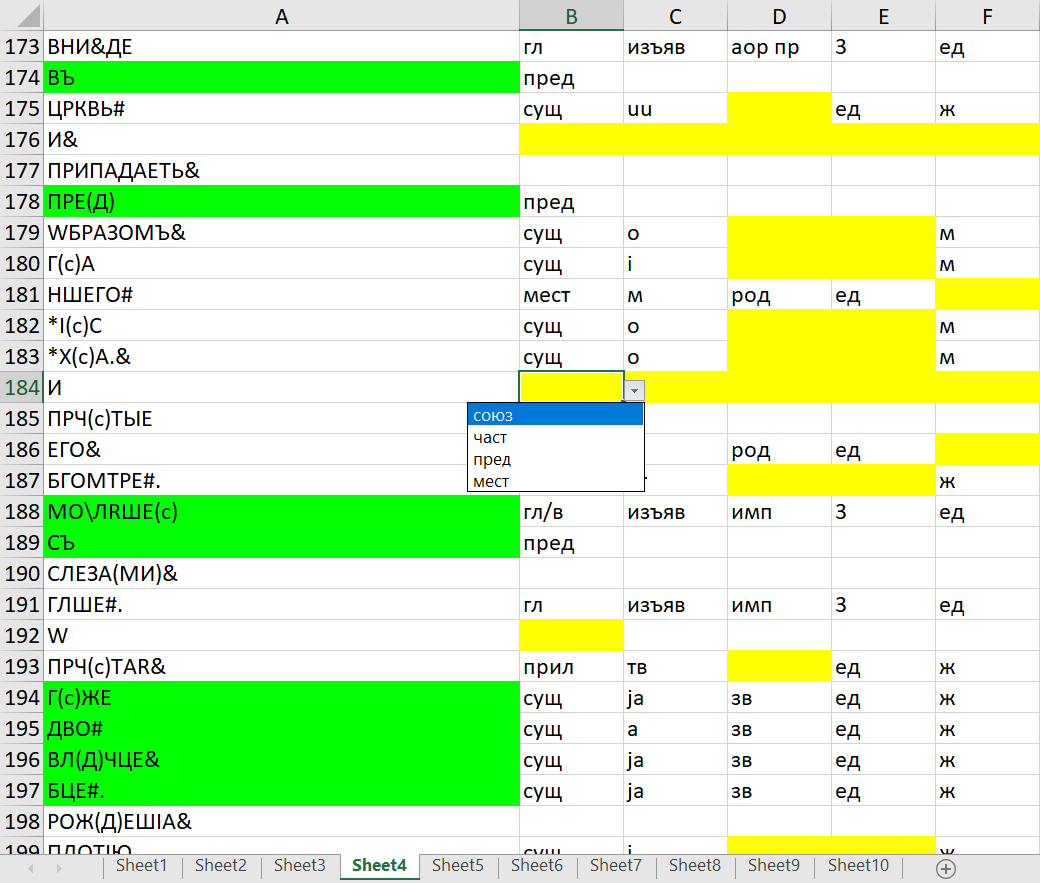
\includegraphics[width=0.6\linewidth]{precedent}
  \end{center}
\end{frame}

\begin{frame}
  \frametitle{Настоящее и будущее проекта}
  \framesubtitle{2010--2020-е~гг.}

  \begin{block}{Высшие уровни}
    \begin{itemize}
      \item разработка форматов синтаксической разметки\autocite{gorlov:2018}
      \item разметка дискурсивных элементов содержания: глав\autocite{rogozina:2015}, цитат\autocite{alexeeva:2019}
    \end{itemize}
  \end{block}
\end{frame}

\begin{frame}
  \frametitle{Настоящее и будущее проекта}
  \framesubtitle{2010--2020-е~гг.}

  \begin{block}{Технологии}
    \begin{itemize}
      \item миграция на платформу TXM: \url{http://textometrie.ens-lyon.fr/}
      \item доступ через интернет --- \foreignlanguage{english}{coming soon}
    \end{itemize}
  \end{block}
\end{frame}
